\chapter{Maintenance, Refactoring \& Code Smells}
\label{ch:maintenance}

More than $60\%$ of total lifecycle cost is spent after the first release. Maintenance is not an afterthought; it is where most engineering effort and business value reside. This chapter covers maintenance categories, refactoring discipline, and the code smells that signal when refactoring is due.

\section{Types of Maintenance}

\begin{itemize}
    \item \textbf{Corrective} --- fix bugs discovered in production (reactive).
    \item \textbf{Adaptive} --- adapt to changes in environment: OS upgrades, library deprecations, regulatory changes.
    \item \textbf{Perfective} --- improve qualities: performance, usability, or add minor enhancements requested by users.
    \item \textbf{Preventive} --- proactively improve structure to prevent future defects (refactoring, adding tests, updating documentation).
\end{itemize}

Lehman's laws observe that useful systems must continually evolve or become progressively less useful, and that each change increases complexity unless work is done to reduce it. Without preventive maintenance, entropy wins.

\begin{figure}[h]
\centering
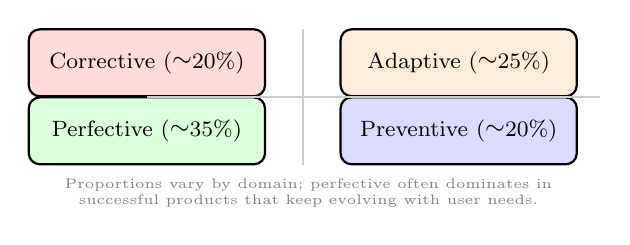
\begin{tikzpicture}[scale=0.72, every node/.style={font=\footnotesize}]
  \tikzstyle{cat}=[draw,rounded corners,minimum width=3.0cm,minimum height=0.85cm,align=center,thick]
  \node[cat,fill=red!14] (corr) at (0,2.2) {Corrective (\raisebox{0.2ex}{\small $\sim$}20\%)};
  \node[cat,fill=orange!14] (adap) at (5.5,2.2) {Adaptive (\raisebox{0.2ex}{\small $\sim$}25\%)};
  \node[cat,fill=green!14] (perf) at (0,1.0) {Perfective (\raisebox{0.2ex}{\small $\sim$}35\%)};
  \node[cat,fill=blue!14] (prev) at (5.5,1.0) {Preventive (\raisebox{0.2ex}{\small $\sim$}20\%)};
  \draw[thick,gray!40] (2.75,0.4) -- (2.75,2.8);
  \draw[thick,gray!40] (0,1.6) -- (8,1.6);
  \node[font=\tiny,gray,align=center] at (2.85,-0.1) {Proportions vary by domain; perfective often dominates in\\successful products that keep evolving with user needs.};
\end{tikzpicture}
\caption{Maintenance categories and typical effort distribution. Investing in preventive work reduces future corrective cost.}
\end{figure}

\section{Refactoring}

\begin{definition}[Refactoring]
A disciplined technique for restructuring existing code, altering its internal structure without changing its external behaviour, to improve readability, reduce complexity, or enable extension.
\end{definition}

Refactoring is not rewriting. Each step is small, behaviour-preserving, and guarded by tests. Classic refactorings include \emph{Extract Method}, \emph{Rename}, \emph{Move Method}, \emph{Replace Conditional with Polymorphism}, and \emph{Introduce Parameter Object}. Fowler's catalogue lists over 60.

\begin{lstlisting}[language=Java,caption={Refactoring: Replace Nested Conditional with Strategy (extract).}]
// Before: long method with branching
double calcPrice(String type, double amt) {
    if (type.equals("REGULAR")) return amt;
    else if (type.equals("VIP")) return amt * 0.8;
    else if (type.equals("STUDENT")) return amt * 0.9;
    else throw new IllegalArgumentException(type);
}
// After: Strategy -- each type is a class, OCP satisfied
interface PricingStrategy { double price(double amt); }
class VipPricing implements PricingStrategy {
    public double price(double amt) { return amt * 0.8; }
}
\end{lstlisting}

When to refactor: before adding a feature that is hard with the current structure (preparatory refactoring), after shipping to clean up, or continuously as part of TDD's refactor step. Never refactor and add behaviour in the same commit---separate the two so failures are attributable.

\section{Code Smells}

Code smells are surface indicators of deeper design problems. They are not bugs, but they predict bugs.

\begin{table}[h]
\centering\small
\begin{tabular}{@{}lp{5.8cm}l@{}}
\toprule
Smell & Symptom & Refactoring \\ \midrule
Long Method & $>30$ lines, many locals & Extract Method \\
Large Class (God Class) & Too many responsibilities & Extract Class \\
Duplicated Code & Same logic in multiple places & Extract Method / Template \\
Long Parameter List & $>4$ parameters & Introduce Parameter Object \\
Feature Envy & Method uses another class more than own & Move Method \\
Data Clumps & Same group of fields recurring & Extract Class \\
Shotgun Surgery & One change touches many classes & Move Method, Inline \\
Primitive Obsession & Primitives for domain concepts & Replace with Value Object \\
\bottomrule
\end{tabular}
\caption{Common code smells and the refactorings that address them.}
\end{table}

\begin{figure}[h]
\centering
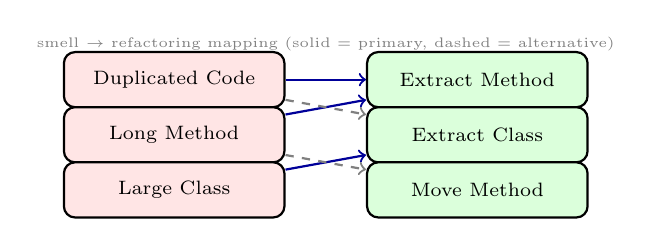
\begin{tikzpicture}[scale=0.70, every node/.style={font=\scriptsize}]
  \tikzstyle{smell}=[draw,rounded corners,fill=red!10,minimum width=2.8cm,minimum height=0.7cm,align=center,thick]
  \tikzstyle{fix}=[draw,rounded corners,fill=green!14,minimum width=2.8cm,minimum height=0.7cm,align=center,thick]
  \node[smell] (dup) at (0,1.6) {Duplicated Code};
  \node[smell] (lm) at (0,0.6) {Long Method};
  \node[smell] (lc) at (0,-0.4) {Large Class};
  \node[fix] (em) at (5.5,1.6) {Extract Method};
  \node[fix] (ec) at (5.5,0.6) {Extract Class};
  \node[fix] (mm) at (5.5,-0.4) {Move Method};
  \draw[->,thick,blue!60!black] (dup) -- (em);
  \draw[->,thick,blue!60!black] (lm) -- (em);
  \draw[->,thick,blue!60!black] (lc) -- (ec);
  \draw[->,thick,dashed,gray] (dup) -- (ec);
  \draw[->,thick,dashed,gray] (lm) -- (mm);
  \node[font=\tiny,gray] at (2.75,2.25) {smell $\to$ refactoring mapping (solid = primary, dashed = alternative)};
\end{tikzpicture}
\caption{Mapping smells to refactorings -- each smell has a preferred remediation; the mapping guides code-review feedback.}
\end{figure}

Detection can be automated: SonarQube, PMD, and Checkstyle flag many smells via metrics (cyclomatic complexity, class size, duplication). But human judgement remains essential---a 40-line method that is perfectly clear is not a smell; a 15-line method with tangled conditionals is.


\section{Reengineering and Migration}

When preventive maintenance is insufficient, \emph{reengineering} systematically transforms a legacy system without changing its functionality: reverse-engineer to recover design, restructure, then forward-engineer. Common strategies include strangler-fig (gradually replace parts behind a facade), branch-by-abstraction (introduce an abstraction layer, migrate incrementally), and big-bang rewrite (high risk, rarely recommended). Migration (e.g., monolith to microservices) follows the same incremental principle: extract one bounded context at a time, with comprehensive contract tests guarding the seam.

\section{Technical Debt}

Technical debt (Cunningham) is the implied cost of future rework caused by choosing an easy, limited solution now instead of a better approach that takes longer. Like financial debt, it accrues interest: every subsequent change is slower. Deliberate, prudent debt (shipping an MVP quickly) can be strategic; inadvertent, reckless debt (copy-pasting without understanding) is corrosive. Manage debt with a visible backlog, allocate $15$--$20\%$ of each iteration to repayment, and track debt via static-analysis metrics.

\begin{lstlisting}[language=Python,caption={Automated smell detection in CI.}]
# Example: fail CI if complexity exceeds threshold
# .github/workflows/quality.yml
# - run: flake8 --max-complexity=10 src/
# - run: sonar-scanner -Dsonar.qualitygate.wait=true
# Quality gate blocks merge when debt ratio exceeds 5%
\end{lstlisting}



\section{Metrics for Maintainability}

Maintainability is measurable. Useful metrics include cyclomatic complexity (McCabe, per method $\leq 10$), cognitive complexity (Sonar, penalises nesting more than linear branches), duplication ratio ($<3\%$), and mean time to change (how long from request to deployed fix). Code churn (lines added/deleted per commit) combined with file age identifies ``hot spots'': frequently changed, complex files that are the best refactoring targets because improvement there pays off most often.

\begin{remark}
Refactoring without tests is just editing. Ensure a green regression suite before restructuring, and keep each refactoring step small enough to be reviewable in under a minute.
\end{remark}

\section{Legacy Code Strategies}

Feathers defines legacy code as code without tests. Strategies for working safely: \emph{sprout} (new behaviour in a new class, called from legacy), \emph{wrap} (extract and test the seam), and \emph{characterisation tests} (write tests that capture current behaviour, even if buggy, before changing it). The goal is to create a safety net incrementally rather than attempting a heroic rewrite.

\section{Change Impact Analysis}

Every maintenance request triggers impact analysis: which requirements, designs, code modules, and tests are affected? Traceability matrices and dependency graphs make this tractable. Techniques include call-graph slicing (what code is reachable from the change), requirements traceability (which REQ-* map to the module), and regression-test selection (run only tests affected by the change for fast feedback, plus full suite nightly). Without analysis, changes cause unintended side effects that surface as production incidents weeks later.

\begin{figure}[h]
\centering
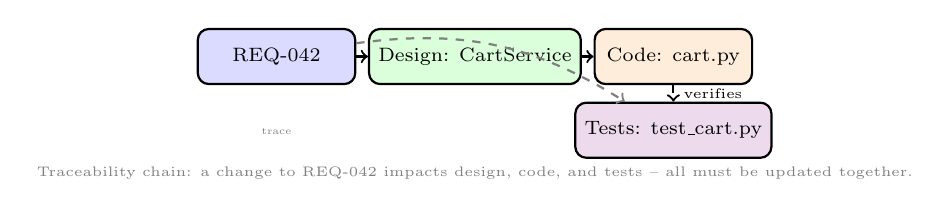
\begin{tikzpicture}[scale=0.72, every node/.style={font=\scriptsize}]
  \tikzstyle{node}=[draw,rounded corners,minimum width=2.0cm,minimum height=0.7cm,align=center,thick]
  \node[node,fill=blue!14] (req) at (0,1.5) {REQ-042};
  \node[node,fill=green!14] (des) at (3.5,1.5) {Design: CartService};
  \node[node,fill=orange!14] (code) at (7.0,1.5) {Code: cart.py};
  \node[node,fill=violet!14] (test) at (7.0,0.2) {Tests: test\_cart.py};
  \draw[->,thick] (req) -- (des);
  \draw[->,thick] (des) -- (code);
  \draw[->,thick,dashed] (code) -- (test) node[midway,right,font=\tiny] {verifies};
  \draw[->,thick,dashed,gray,bend left=20] (req) to (test) node[midway,above,font=\tiny] {trace};
  \node[font=\tiny,gray,align=center] at (3.5,-0.55) {Traceability chain: a change to REQ-042 impacts design, code, and tests -- all must be updated together.};
\end{tikzpicture}
\caption{Impact analysis via traceability -- a requirement change propagates through design, code, and tests; missing any link is a defect.}
\end{figure}


\section{Documentation and Knowledge Transfer}

Outdated documentation is worse than none: it misleads. Treat docs as code---versioned, reviewed, and tested (e.g., doctests that verify examples still run). Onboarding guides, ADRs, and runbooks (operational playbooks) are the highest-value docs for maintenance. When a senior developer leaves, their undocumented knowledge leaves with them; pair programming and written ADRs mitigate this bus-factor risk.


\section{Estimating Maintenance Effort}

Maintenance effort is estimated differently from greenfield: use change-impact size (lines or points affected), historical velocity for similar changes, and a risk multiplier for poorly understood legacy areas. Planning poker should include a ``unknown'' card that triggers a time-boxed spike before committing to an estimate. Underestimation is the norm when impact analysis is skipped.

\begin{remark}
Every hour spent on preventive maintenance (tests, refactoring, docs) saves multiple hours of future corrective work. The difficulty is that the saving is invisible until the crisis that did not happen.
\end{remark}

\begin{figure}[h]
\centering
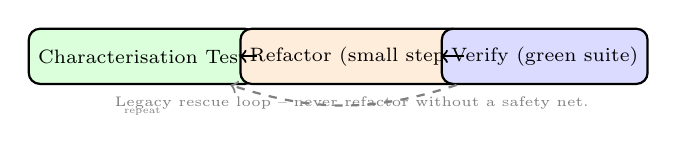
\begin{tikzpicture}[scale=0.70, every node/.style={font=\scriptsize}]
  \tikzstyle{b}=[draw,rounded corners,minimum width=2.2cm,minimum height=0.7cm,align=center,thick]
  \node[b,fill=green!14] (a) at (0,1.2) {Characterisation Test};
  \node[b,fill=orange!14] (b) at (3.8,1.2) {Refactor (small step)};
  \node[b,fill=blue!14] (c) at (7.3,1.2) {Verify (green suite)};
  \draw[->,thick] (a) -- (b); \draw[->,thick] (b) -- (c);
  \draw[->,thick,dashed,gray,bend left=18] (c) to (a) node[midway,above,font=\tiny] {repeat};
  \node[font=\tiny,gray] at (3.8,0.35) {Legacy rescue loop -- never refactor without a safety net.};
\end{tikzpicture}
\caption{Safe refactoring loop for legacy code: capture behaviour first, then restructure incrementally.}
\end{figure}

\section{Exercises}

\begin{exercise}
Classify each maintenance request: (a) fix crash on empty cart, (b) migrate from Java~11 to 17, (c) add dark mode, (d) extract duplicated payment logic. Which Lehman law does (d) address?
\end{exercise}

\begin{exercise}
A method has cyclomatic complexity 18 and 60~lines with four levels of nesting. Identify the smells, propose a refactoring sequence (two steps), and explain how you would verify behaviour is preserved.
\end{exercise}

\begin{exercise}
Distinguish refactoring from rewriting. Why should refactoring commits be kept separate from feature commits? Give a scenario where mixing them hides a bug.
\end{exercise}

\begin{exercise}
Your team has $30\%$ duplicated code by line count. Propose a concrete, incremental plan to reduce it to $<10\%$ over four iterations without halting feature work. What metrics would you track?
\end{exercise}

\begin{exercise}
Explain technical debt with a financial analogy. Give one example of prudent deliberate debt and one of reckless inadvertent debt in a university project context.
\end{exercise}
